\subsubsection{26.12.2015}
\textit{\textbf{Time frame:}} 16:00-22:00 \newline
On the ramp for debris there were installed special walls for leading scoring elements to the entrance of the bucket.
A second pair of shores for the prevention of the entanglement of the cables on the winch coil was installed.
There used to be a problem that slats, on which the bucket is mounted, bend a lot under it's weight. This day it was found a solution to this problem: it is possible to install a special band, that will be fixed on the top slat and slide along the surface to which the bottom slat is attached. This band will rest in the surface and prevent construction from bending.
Today it was created a prototype of this module.

\begin{figure}[H]
	\begin{minipage}[h]{0.58\linewidth}
		\center{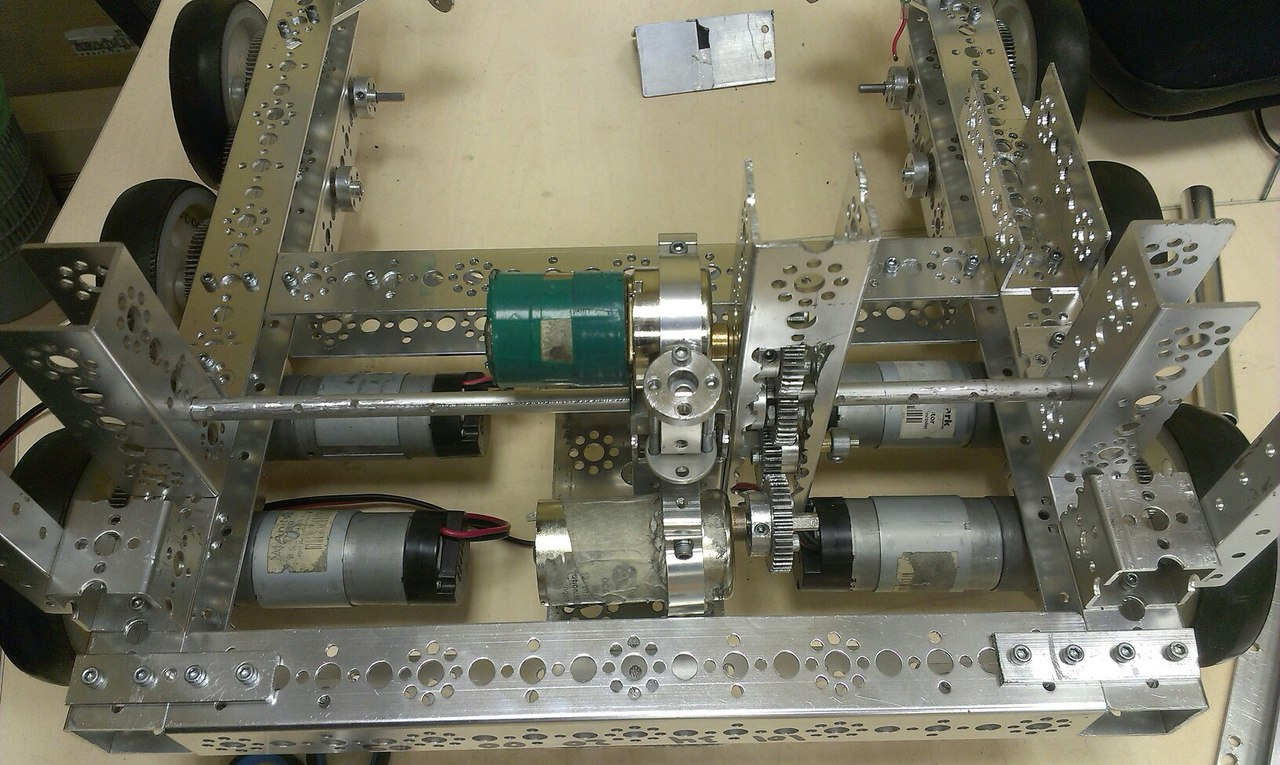
\includegraphics[scale=0.2]{3Engineering/5Team_meetings/days_of_meetings/2015.12.17/images/01}}
		\caption{Winch installed onto the carriage}
	\end{minipage}
	\hfill
	\begin{minipage}[h]{0.37\linewidth}
		\center{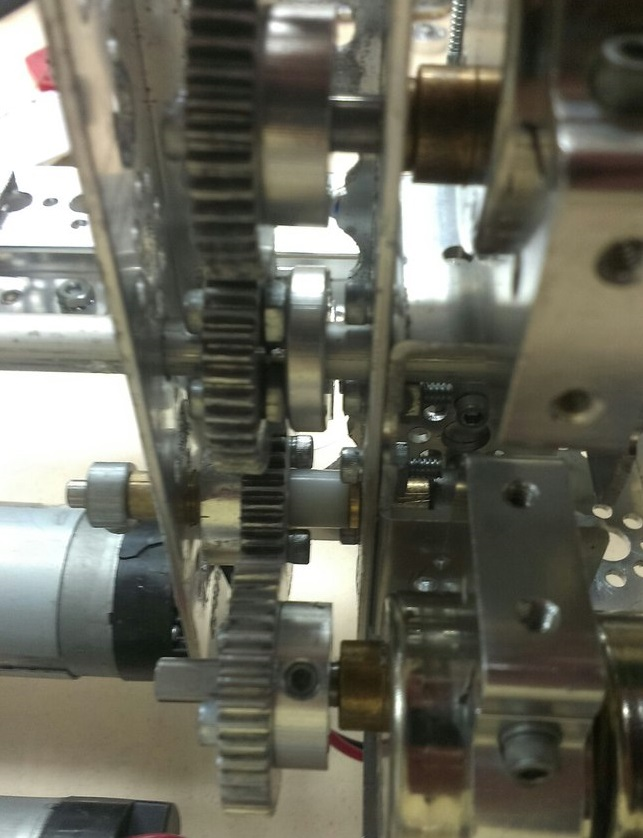
\includegraphics[scale=0.22]{3Engineering/5Team_meetings/days_of_meetings/2015.12.17/images/02}}
		\caption{The construction of the winch}
	\end{minipage}
\end{figure}
